\documentclass[a4paper,11pt]{article}
\usepackage{ctex}
\usepackage{enumerate}
\usepackage{times}
\usepackage{mathptmx}
\usepackage{amsmath}
\usepackage{amssymb}
\usepackage{tikz}
\usepackage[top=2cm, bottom=2cm, left=2cm, right=2cm]{geometry}

\allowdisplaybreaks[4]
\renewcommand{\labelenumi}{(\alph{enumi})}
\newcommand{\set}[1]{\{#1\}}
\newcommand{\diam}{\mathop{\mathrm{diam}}}
\begin{document}
  \title{����~2-15~��ҵ}
  \author{��������ۿԴ \and ѧ�ţ�161240004}
  \date{}
  \maketitle

  \section{[CZ] Problem 1.6}
  \small
  \begin{centering}
    \begin{tikzpicture}[line width = 1pt,
                      solid/.style = {circle, draw, fill = black, minimum size = 0.1cm},
                      empty/.style = {circle, draw, fill = white, minimum size = 0.1cm}]
    \node [empty, label=above:$c_1$] (c1) at (1, 1){};
    \node [empty, label=above:$c_2$] (c2) at (2, 1){};
    \node [empty, label=above:$c_3$] (c3) at (3, 1){};
    \node [empty, label=above:$c_4$] (c4) at (4, 1){};
    \node [empty, label=above:$c_5$] (c5) at (5, 1){};
    \node [empty, label=above:$c_6$] (c6) at (6, 1){};
    \node [empty, label=below:$c_7$] (c7) at (1, 0){};
    \node [empty, label=below:$c_8$] (c8) at (2, 0){};
    \node [empty, label=below:$c_9$] (c9) at (3, 0){};
    \node [empty, label=below:$c_{10}$] (c10) at (4, 0){};
    \node [empty, label=below:$c_{11}$] (c11) at (5, 0){};
    \node [empty, label=below:$c_{12}$] (c12) at (6, 0){};

    \draw (c1) edge [bend left=30] (c5);
    \draw (c1) edge [bend left=45] (c6);
    \draw (c1) -- (c8);
    \draw (c1) -- (c9);
    \draw (c2) -- (c7);
    \draw (c2) -- (c10);
    \draw (c3) -- (c7);
    \draw (c3) -- (c10);
    \draw (c4) -- (c8);
    \draw (c4) -- (c9);
    \draw (c4) -- (c11);
    \draw (c4) -- (c12);
    \draw (c5) -- (c10);
    \draw (c6) -- (c10);
    \draw (c7) edge [bend right=30] (c11);
    \draw (c7) edge [bend right=45p] (c12);
    \end{tikzpicture} \par
  \end{centering}
  \normalsize
  \section{[CZ] Problem 1.8}
  \begin{enumerate}
    \item The words in $S_1$ are (presented from left to right): cat, cap, tap, top. \par
    The words in $S_2$ are: map (center) , mop, tap, mat (surrounding). \par
    The words in $S_3$ are: run (top left), gun (top right), sun (center), son (bottom). \par
    The words in $S_4$ are (presented clockwise): slit, slot, slop, slip. \par
    The words in $S_5$ are (presented clockwise from top left): pot, put, pet, poet. \par
    The words in $S_6$ are (presented clockwise): lake, sake, take, make.
    \item  The graph $H$ is: \par
      \small
      \begin{centering}
      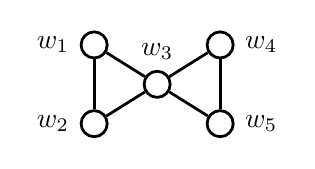
\begin{tikzpicture}[line width = 1pt,
                        solid/.style = {circle, draw, fill = black, minimum size = 0.1cm},
                        empty/.style = {circle, draw, fill = white, minimum size = 0.1cm}]
      \node [empty, label=left:$w_1$] (T1) at (0, 1){};
      \node [empty, label=left:$w_2$] (T2) at (0, 0){};
      \node [empty, label=above:$w_3$] (T3) at (0.8, 0.5){};
      \node [empty, label=right:$w_4$] (T4) at (1.6, 1){};
      \node [empty, label=right:$w_5$] (T5) at (1.6, 0){};

      \draw (T1) -- (T2);
      \draw (T4) -- (T5);
      \draw (T1) -- (T3) -- (T4);
      \draw (T2) -- (T3) -- (T5);
      \end{tikzpicture} \par
      \end{centering}
      \normalsize
      It is a word graph of some set, and the corresponding words are: top, tap, tip, lip, dip.
  \end{enumerate}

  \section{[CZ] Problem 1.10}
  \small
  \begin{centering}
  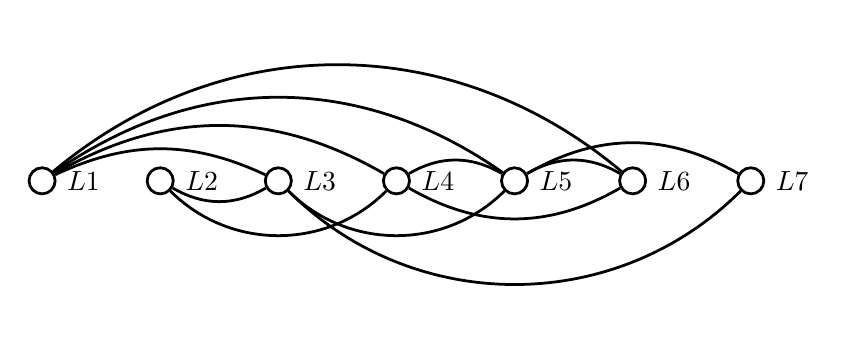
\begin{tikzpicture}[line width = 1pt,
                    solid/.style = {circle, draw, fill = black, minimum size = 0.1cm},
                    empty/.style = {circle, draw, fill = white, minimum size = 0.1cm}]
  \node [empty, label=right:$L1$] (L1) at (0, 0){};
  \node [empty, label=right:$L2$] (L2) at (1.5, 0){};
  \node [empty, label=right:$L3$] (L3) at (3, 0){};
  \node [empty, label=right:$L4$] (L4) at (4.5, 0){};
  \node [empty, label=right:$L5$] (L5) at (6, 0){};
  \node [empty, label=right:$L6$] (L6) at (7.5, 0){};
  \node [empty, label=right:$L7$] (L7) at (9, 0){};

  \draw (L1) edge [bend left=25] (L3);
  \draw (L1) edge [bend left=30] (L4);
  \draw (L1) edge [bend left=35] (L5);
  \draw (L1) edge [bend left=40] (L6);
  \draw (L2) edge [bend right=30] (L3);
  \draw (L2) edge [bend right=45] (L4);
  \draw (L3) edge [bend right=45] (L5);
  \draw (L3) edge [bend right=45] (L7);
  \draw (L4) edge [bend left=30] (L5);
  \draw (L5) edge [bend left=30] (L6);
  \draw (L5) edge [bend left=30] (L7);
  \draw (L4) edge [bend right=30] (L6);
  \end{tikzpicture} \par
  \end{centering}
  \normalsize

  \section{[CZ] Problem 1.14}
  Let $C$ denote a component of $G$. \par
  (1) $\rightarrow$ (2): Take any vertex $v_0$ in $C$. For any vertex $v_i$ which is connected to $v_0$, it must in $V(C)$, otherwise if we add $v_i$, along with the edges in the path from $v_0$ to $v_i$, to $C$, we get a proper connected supergraph of $C$, which leads to contradiction. Therefore, $V(C)$ is an equivalent class. Then we have to prove $C$ is the subgraph induced by $V(C)$. If not, let $C'$ be the subgraph induced by $V(C)$, and $E(C) \subset E(C')$, thus $C$ is a proper subgraph of $C'$, which leads to contradiction.  \par
  (2) $\rightarrow$ (1): Suppose, to the contrary that $C$ is a proper subgraph of a connected subgraph of $G$, denoted by $C'$. If $V(C) \subset V(C')$, there exists some vertex connected to $C$ but not in the equivalent class, which leads to contradiction. It is impossible that $V(C) = V(C')$, because the subgraph induced by $V(C)$ is the maximal subgraph whose vertex set is $V(C)$.

  \section{[CZ] Problem 1.16}
  For every $i$, we have a path from $u$ to $v_i$: $(u = v_0, v_1, \cdots, v_i)$, whose length is $i$. Thus $d(u, v_i) \leq i$. \par
  Suppose, to the contrary that $d(u, v_i) < i$, i.e. there exists path $(u_0 = v_0, u_1, \cdots, u_j = v_i)$, where $j < i$. Consider the walk $(u = u_0 = v_0, u_1, \cdots, u_j = v_i, v_{i+1}, \cdots, v_k = v)$, it's a $u-v$ walk shorter than the geodesic, which leads to contradiction. \par
  Therefore, $d(u, v_i) = i$ for each integer $i$ with $1 \leq i \leq k$.

  \section{[CZ] Problem 1.17}
  \begin{enumerate}
    \item Assume that $P$ is an $x - z$ path and $Q$ is a $u - w$ path, where $x \neq u, v$ and $y \neq u, v$, and they do not have common vertex. Let $y$ be a vertex in $P$ and $v$ be a vertex in $Q$, then there exists a $y-v$ path $(p_0 = y, p_1, p_2, \cdots, p_n = v)$. If there exists $p_i$ such that $p_i$ ($0 < i < n$) is in $P$ or $Q$, since $P \cap Q = \varnothing$, there exists a segment of the path, from any vertex in $P$ (let it be $y$), to any vertex in $Q$ (let it be $v$), such that the vertices in the segment are not in $P$ or $Q$, except the first and the last one. Assume $x - y$ is longer than $y - z$, and $u - v$ is longer than $v - w$, consider the path $x - y - v - u$, it is longer than the $x - z$ path and the $u - v$ path, which leads to contradiction.
    \item This is true. The geodesics are as well the longest paths in $G$, otherwise $\diam(G) > k$. Apply the conclusion we've proved in (1), we obtain that $P$ and $Q$ must have at least one common vertex.
  \end{enumerate}

  \section{[CZ] Problem 1.18}
  \begin{enumerate}
    \item The minimum size of such a subgraph contains only the vertices and edges in a $u-v$ geodesic. Any connected subgraph containing $u$ and $v$ must have a $u-v$ path, which is at least as long as the geodesic. So a subgraph contains only the vertices and edges in a $u-v$ geodesic has less edges or vertices than other graphs.
    \item What is the maximum size of a connected subgraph of $G$ containing $u$ and $v$? It is $G$.
  \end{enumerate}

  \section{[CZ] Problem 1.22}
  If $u, v$ are in two different components of $G$, then $uv \in E(\overline{G})$, i.e. $d_{\overline{G}}(u, v) = 1$. \par
  If $u, v$ are in the same component of $G$, let $w$ be a vertex in another component $G$. We have $uw, wv \in E(\overline{G})$, i.e. $(u, w, v)$ is a path from $u$ to $v$, and thus $d_{\overline{G}}(u, v) \leq 2$. \par
  Therefore, $d_{\overline{G}}(u, v) = 1$ or $d_{\overline{G}}(u, v) = 2$.

  \section{[CZ] Problem 1.23}
  \begin{enumerate}
  \item For $k = 1$, the graph $G = (V, E)$ is: \par
      \small
      \begin{centering}
      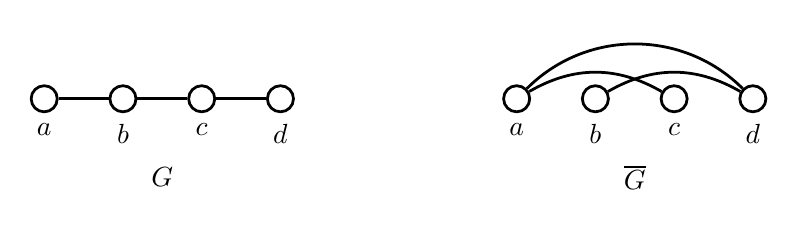
\begin{tikzpicture}[line width = 1pt,
                        solid/.style = {circle, draw, fill = black, minimum size = 0.1cm},
                        empty/.style = {circle, draw, fill = white, minimum size = 0.1cm}]
      \node [empty, label=below:$a$] (a) at (0, 0){};
      \node [empty, label=below:$b$] (b) at (1, 0){};
      \node [empty, label=below:$c$] (c) at (2, 0){};
      \node [empty, label=below:$d$] (d) at (3, 0){};
      \node at (1.5, -1) {$G$};

      \draw (a) -- (b) -- (c) -- (d);

      \node [empty, label=below:$a$] (a) at (6, 0){};
      \node [empty, label=below:$b$] (b) at (7, 0){};
      \node [empty, label=below:$c$] (c) at (8, 0){};
      \node [empty, label=below:$d$] (d) at (9, 0){};
      \node at (7.5, -1) {$\overline{G}$};

      \draw (a) edge [bend left=30] (c);
      \draw (b) edge [bend left=30] (d);
      \draw (a) edge [bend left=45] (d);

      \end{tikzpicture} \par
      \end{centering}
      \normalsize
    and $d_{G}(b, c) = 1 = d_{\overline{G}}(a, d)$. \par

    For $k = 2$, the graph $G = (V, E)$ is\par
      \small
      \begin{centering}
      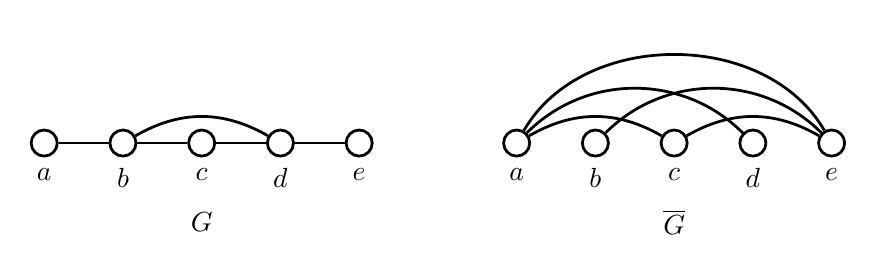
\begin{tikzpicture}[line width = 1pt,
                        solid/.style = {circle, draw, fill = black, minimum size = 0.1cm},
                        empty/.style = {circle, draw, fill = white, minimum size = 0.1cm}]
      \node [empty, label=below:$a$] (a) at (0, 0){};
      \node [empty, label=below:$b$] (b) at (1, 0){};
      \node [empty, label=below:$c$] (c) at (2, 0){};
      \node [empty, label=below:$d$] (d) at (3, 0){};
      \node [empty, label=below:$e$] (e) at (4, 0){};
      \node at (2, -1) {$G$};

      \draw (a) -- (b) -- (c) -- (d) -- (e);
      \draw (b) edge [bend left=30] (d);

      \node [empty, label=below:$a$] (a) at (6, 0){};
      \node [empty, label=below:$b$] (b) at (7, 0){};
      \node [empty, label=below:$c$] (c) at (8, 0){};
      \node [empty, label=below:$d$] (d) at (9, 0){};
      \node [empty, label=below:$e$] (e) at (10, 0){};
      \node at (8, -1) {$\overline{G}$};

      \draw (a) edge [bend left=30] (c);
      \draw (a) edge [bend left=45] (d);
      \draw (a) edge [bend left=60] (e);
      \draw (b) edge [bend left=45] (e);
      \draw (c) edge [bend left=30] (e);
      \end{tikzpicture} \par
      \end{centering}
      \normalsize
    and $d_{G}(a, d) = 2 = d_{\overline{G}}(b, c)$.
  \item The largest value of $k$ is 3. Here is an example when $k = 3$, $d_G(a_0, a_3) = 3 = d_{\overline{G}}(b_0, b_3)$:\par
      \small
      \begin{centering}
      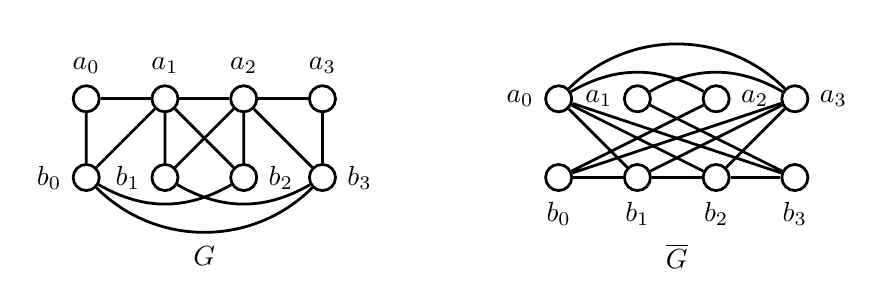
\begin{tikzpicture}[line width = 1pt,
                        solid/.style = {circle, draw, fill = black, minimum size = 0.1cm},
                        empty/.style = {circle, draw, fill = white, minimum size = 0.1cm}]
      \node [empty, label=above:$a_0$] (a0) at (0, 0){};
      \node [empty, label=above:$a_1$] (a1) at (1, 0){};
      \node [empty, label=above:$a_2$] (a2) at (2, 0){};
      \node [empty, label=above:$a_3$] (a3) at (3, 0){};

      \node [empty, label=left:$b_0$] (b0) at (0, -1){};
      \node [empty, label=left:$b_1$] (b1) at (1, -1){};
      \node [empty, label=right:$b_2$] (b2) at (2, -1){};
      \node [empty, label=right:$b_3$] (b3) at (3, -1){};

      \node at (1.5, -2) {$G$};

      \draw (a0) -- (a1) -- (a2) -- (a3);
      \draw (a0) -- (b0) -- (a1) -- (b2) -- (a2);
      \draw (a1) -- (b1) -- (a2) -- (b3) -- (a3);
      \draw (b0) edge [bend right=30] (b2);
      \draw (b1) edge [bend right=30] (b3);
      \draw (b0) edge [bend right=45] (b3);

      \node [empty, label=left:$a_0$] (a0) at (6, 0){};
      \node [empty, label=left:$a_1$] (a1) at (7, 0){};
      \node [empty, label=right:$a_2$] (a2) at (8, 0){};
      \node [empty, label=right:$a_3$] (a3) at (9, 0){};

      \node [empty, label=below:$b_0$] (b0) at (6, -1){};
      \node [empty, label=below:$b_1$] (b1) at (7, -1){};
      \node [empty, label=below:$b_2$] (b2) at (8, -1){};
      \node [empty, label=below:$b_3$] (b3) at (9, -1){};

      \draw (b0) -- (b1) -- (b2) -- (b3);
      \draw (a0) -- (b1) -- (a3);
      \draw (a0) -- (b2) -- (a3);
      \draw (a0) -- (b3) -- (a1);
      \draw (a2) -- (b0) -- (a3);
      \draw (a0) edge [bend left=30] (a2);
      \draw (a1) edge [bend left=30] (a3);
      \draw (a0) edge [bend left=45] (a3);

      \node at (7.5, -2) {$\overline{G}$};
      \end{tikzpicture} \par
      \end{centering}
      \normalsize
      Now we are going to prove that it is impossible that $k \geq 4$. Suppose, there exists distinct $u, v, x, y$, such that $d_G(u, v) = d_{\overline{G}}(x,y) = k \geq 4$. Let $(u = w_0, w_1, \cdots, w_k = v)$ be a $u-v$ geodesic, $(x = z_0, z_1, \cdots, z_k = y)$ be an $x-y$ geodesic. We claim that there exists $i \in \set{0,k}$, such that $z_0 w_i$ is not an edge in $G$, otherwise, $(w_0, z_0, w_k)$ is a $u-v$ path shorter than the geodesic in $G$. Likewise there exists $j \in \set{0,k}$, such that $z_k w_j$ is not an edge in $G$. Hence, $z_0 w_i$ and $z_k w_j$ are edges in $\overline{G}$. If $i = j$, $(z_0, w_i, z_k)$ is shorter than $x-y$ geodesic, which is impossible. If $i \neq j$, $w_i w_j = w_0 w_k = u v$ is an edge in $\overline{G}$, otherwise $d_G(u, v) = 1$, contradicting the provided condition. Note that $(x = z_0, w_i, w_j, z_k = y)$ is an $x-y$ path shorter than the geodesic, which is impossible. \par
      Therefore, $k \leq 3$.
  \end{enumerate}

  \section{[CZ] Problem 1.25}
  Assume that $G$ is bipartite, with partite sets $U$ and $W$. Since $|V(G)| = |U| + |W| \geq 5$, at least one of $|U|$ and $|G|$ is greater than 2. Assume, without loss of generality, that $|U| \geq 3$. Let $u, v, w$ be three distinct vertices in $U$. They are mutually adjacent in $\overline{G}$, which forms an odd cycle. By Theorem 1.12, $\overline{G}$ is not bipartite. \par
  Therefore, if $|V(G)| \geq 5$, at most one of $G$ and $\overline{G}$ is bipartite.

  \section{[CZ] Problem 1.30}
  \small
  \begin{centering}
    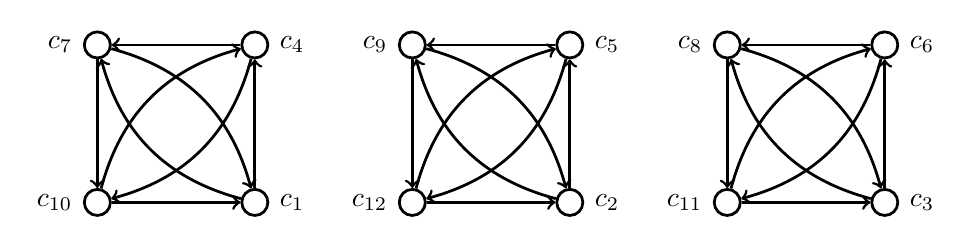
\begin{tikzpicture}[line width = 1pt,
                      solid/.style = {circle, draw, fill = black, minimum size = 0.1cm},
                      empty/.style = {circle, draw, fill = white, minimum size = 0.1cm}]
    \node [empty, label=right:$c_1$] (c1) at (0, 0){};
    \node [empty, label=right:$c_4$] (c4) at (0, 2){};
    \node [empty, label=left:$c_7$] (c7) at (-2, 2){};
    \node [empty, label=left:$c_{10}$] (c10) at (-2, 0){};
    \draw[->] (c1) -- (c4);
    \draw[->] (c4) -- (c7);
    \draw[->] (c7) -- (c10);
    \draw[->] (c10) -- (c1);
    \draw[->] (c1) edge [bend left=30] (c7);
    \draw[->] (c7) edge [bend left=30] (c1);
    \draw[->] (c4) edge [bend left=30] (c10);
    \draw[->] (c10) edge [bend left=30] (c4);

    \node [empty, label=right:$c_2$] (c2) at (4, 0){};
    \node [empty, label=right:$c_5$] (c5) at (4, 2){};
    \node [empty, label=left:$c_9$] (c9) at (2, 2){};
    \node [empty, label=left:$c_{12}$] (c12) at (2, 0){};
    \draw[->] (c2) -- (c5);
    \draw[->] (c5) -- (c9);
    \draw[->] (c9) -- (c12);
    \draw[->] (c12) -- (c2);
    \draw[->] (c2) edge [bend left=30] (c9);
    \draw[->] (c9) edge [bend left=30] (c2);
    \draw[->] (c5) edge [bend left=30] (c12);
    \draw[->] (c12) edge [bend left=30] (c5);

    \node [empty, label=right:$c_3$] (c3) at (8, 0){};
    \node [empty, label=right:$c_6$] (c6) at (8, 2){};
    \node [empty, label=left:$c_8$] (c8) at (6, 2){};
    \node [empty, label=left:$c_{11}$] (c11) at (6, 0){};
    \draw[->] (c3) -- (c6);
    \draw[->] (c6) -- (c8);
    \draw[->] (c8) -- (c11);
    \draw[->] (c11) -- (c3);
    \draw[->] (c3) edge [bend left=30] (c8);
    \draw[->] (c8) edge [bend left=30] (c3);
    \draw[->] (c6) edge [bend left=30] (c11);
    \draw[->] (c11) edge [bend left=30] (c6);
    \end{tikzpicture} \par
  \end{centering}
  \normalsize

  \section{[CZ] Problem 1.31}
  Define that, $(c_i, c_j)$ is a directed edge, if and only if $c_j$ can be obtained from $c_i$ by rotating the configuration $90^\circ$ clockwise, and then interchanging the two coins. The graph is: \par
  \vspace{0.2cm}
  \small
  \begin{centering}
    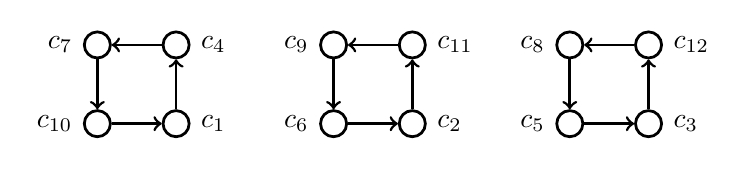
\begin{tikzpicture}[line width = 1pt,
                      solid/.style = {circle, draw, fill = black, minimum size = 0.1cm},
                      empty/.style = {circle, draw, fill = white, minimum size = 0.1cm}]
    \node [empty, label=right:$c_1$] (c1) at (0, 0){};
    \node [empty, label=right:$c_4$] (c10) at (0, 1){};
    \node [empty, label=left:$c_7$] (c7) at (-1, 1){};
    \node [empty, label=left:$c_{10}$] (c4) at (-1, 0){};
    \draw[->] (c1) -- (c10);
    \draw[->] (c10) -- (c7);
    \draw[->] (c7) -- (c4);
    \draw[->] (c4) -- (c1);

    \node [empty, label=right:$c_2$] (c2) at (3, 0){};
    \node [empty, label=right:$c_{11}$] (c11) at (3, 1){};
    \node [empty, label=left:$c_9$] (c9) at (2, 1){};
    \node [empty, label=left:$c_6$] (c6) at (2, 0){};
    \draw[->] (c2) -- (c11);
    \draw[->] (c11) -- (c9);
    \draw[->] (c9) -- (c6);
    \draw[->] (c6) -- (c2);

    \node [empty, label=right:$c_3$] (c3) at (6, 0){};
    \node [empty, label=right:$c_{12}$] (c12) at (6, 1){};
    \node [empty, label=left:$c_8$] (c8) at (5, 1){};
    \node [empty, label=left:$c_5$] (c5) at (5, 0){};
    \draw[->] (c3) -- (c12);
    \draw[->] (c12) -- (c8);
    \draw[->] (c8) -- (c5);
    \draw[->] (c5) -- (c3);
    \end{tikzpicture} \par
  \end{centering}
  \normalsize

  \section{[CZ] Problem 2.6}
  Consider the sum of the degrees over all vertices:
  $$\sum_{v \in V(G)} \deg v = n(n-1) + n^2 + n(n+1) = 3n^2$$
  By Theorem 2.1, $3n^2$ is even, thus $n$ is even.

  \section{[CZ] Problem 2.7}
  \begin{enumerate}
    \item For every $v \in V(G)$, by the definition of bipartite graph, one of its incident vertices is in $U$, the other is in $W$. Therefore $m = \sum_{u \in U} \deg u = \sum_{w \in W} \deg w$.
    \item Let $x$ be the number of vertices of $G$ having degree 2. Then we have the following equation
    \begin{align*}
      \sum_{u \in U} \deg u &= \sum_{w \in W} \deg w \\
      3 \times |U| &= 2 \times n + 4 \times (|W| - n)
    \end{align*}
    After some algebra we get $n = 2$.
  \end{enumerate}

  \section{[CZ] Problem 2.9}
  Suppose that these odd vertices are not in the same component. Let $C$ be the component containing only one odd vertex. Component is an induced subgraph, so the degrees of its vertices do not change. The sum of the degrees over all vertices in $C$ is odd, which contradicts Theorem 2.1. \par

  \section{[CZ] Problem 2.10}
  \begin{enumerate}
    \item Let $K_a, K_b$ be two complete graph with degrees $a$ and $b$, where $a, b \geq 2$ and $a + b = n$. Let $u, v$ be any vertices in $K_a$ and $K_b$, respectively. Connect the two graphs by edge $uv$, we get a new connected graph $G$. For every nonadjacent vertices $x, y$, they are in two different complete graphs and $\set{x,y} \neq \set{u,v}$, otherwise they are adjacent. Assume that $x \in K_a$ and $y \in K_b$. If $x = u$ or $y = v$, $\deg x + \deg y = n-1$, otherwise $\deg x + \deg y = n-2$.
    \item If the graph has more than one components, remove any one of them. The remaining part of the graph has at most $n-1$ vertices, with $\deg u + \deg v \geq n - 2$ still holds. By Theorem 2.4, it is connected. Therefore, $G$ has at most two components.
    \item No. Instead of moving any component, we remove the one with greater order. The remaining part of the graph has at most $\lfloor n/2 \rfloor$ vertices. If $\deg u + \deg v \geq \lfloor n/2 \rfloor - 1$ for all nonadjacent $u, v$, the remaining part is connected. Thus $\lfloor n/2 \rfloor - 1$ is a shaper bound.
  \end{enumerate}

  \section{[CZ] Problem 2.13}
  \begin{enumerate}
    \item Suppose, to the contrary that $G$ contains more than two components. The component containing minimum number of vertices contains at most $\lfloor n/3 \rfloor$ vertices. The degree of every vertex in this component is at most $\lfloor n/3 \rfloor - 1$, less than $(n-2)/3$, which leads to contradiction.
    \item If $\deg v \geq (n-3)/3 = n/3 - 1$ for every vertex $v$ of $G$, $G$ might contain more than two components. For example, let $n$ be a multiple of 3, consider the graph $G = 3K_{n/3}$, for every $v \in V(G)$, $\deg v = n/3 - 1$, however, it contains three components.
  \end{enumerate}

  \section{[CZ] Problem 2.15}
  For every cycle in graph $G$, let $u, v$ be two distinct vertices in the cycle, and thus the cycle consists two $u-v$ path, whose lengths have the same parity. Therefore the cycle is an even cycle. By Theorem 1.12 $G$ is bipartite.

  \section{[CZ] Problem 2.20}
  Suppose, to the contrary that for every adjacent vertices $u$ and $v$, $\deg u = \deg v$. Since the graph is connected, for every distinct vertices $x$ and $y$, there exists an $x - y$ path. By transitivity of ``$=$'', we get $\deg x = \deg y$, i.e. $G$ is regular, which leads to contradiction.

  \section{[CZ] Problem 2.25}
  \begin{enumerate}
    \item By Theorem 2.1, $\sum_{u \in V(G)} \deg u$ is even, thus $G-v$ has even order, therefore $G$ has odd order.
    \item Suppose, to the contrary, that there exists some component of odd order, denoted by $C$. Consider
    $$ \sum_{v \in V(C)} \deg v = r |V(C)|$$
    it is odd, which contradicts Theorem 2.1. Therefore, $G$ does not contain any component of odd order.
  \end{enumerate}

  \section{[CZ] Problem 2.27}
  For bipartite graph, we have $\sum_{u \in U} \deg u = \sum_{w \in W} \deg w$, so $r|U| = r|W|$. Eliminating $r$ yields $|U| = |W|$.

  \section{[CZ] Problem 2.28}
  Yes. When $G$ itself is an $r$-regular graph, the graph $H$ in Theorem 2.7 is equal to $G$, which of course has the smallest order.

  \section{[CZ] Problem 3.6}
  No. Consider the two graphs \par
  \vspace{0.2cm}
  \small
  \begin{centering}
    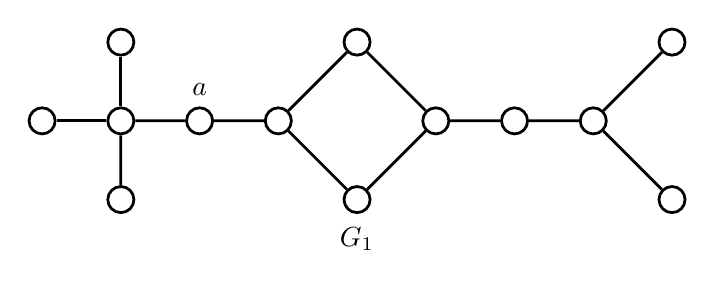
\begin{tikzpicture}[line width = 1pt,
                      solid/.style = {circle, draw, fill = black, minimum size = 0.1cm},
                      empty/.style = {circle, draw, fill = white, minimum size = 0.1cm}]
    \node [empty] (a1) at (1, 1){};
    \node [empty] (a2) at (0, 0){};
    \node [empty] (a3) at (1, -1){};
    \node [empty] (a4) at (1, 0){};
    \node [empty, label=above:$a$] (a5) at (2, 0){};
    \node [empty] (a6) at (3, 0){};
    \node [empty] (a7) at (4, 1){};
    \node [empty] (a8) at (4, -1){};
    \node [empty] (a9) at (5, 0){};
    \node [empty] (a10) at (6, 0){};
    \node [empty] (a11) at (7,0){};
    \node [empty] (a12) at (8, 1){};
    \node [empty] (a13) at (8, -1){};

    \draw (a1) -- (a4) -- (a2);
    \draw (a3) -- (a4) -- (a5) -- (a6) -- (a8) -- (a9) -- (a10) -- (a11) -- (a12);
    \draw (a6) -- (a7) -- (a9);
    \draw (a11) -- (a13);
    \node at (4, -1.5) {$G_1$};
    \end{tikzpicture} \par
    \vspace{0.2cm}
    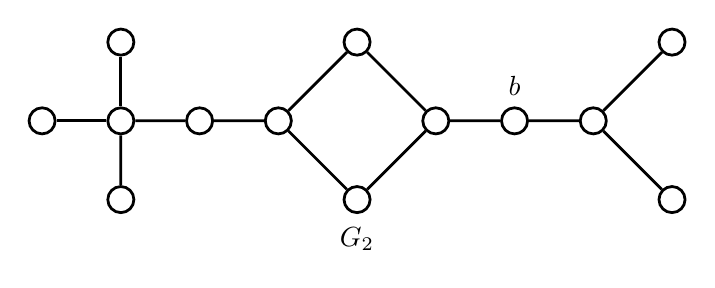
\begin{tikzpicture}[line width = 1pt,
                      solid/.style = {circle, draw, fill = black, minimum size = 0.1cm},
                      empty/.style = {circle, draw, fill = white, minimum size = 0.1cm}]
    \node [empty] (a1) at (1, 1){};
    \node [empty] (a2) at (0, 0){};
    \node [empty] (a3) at (1, -1){};
    \node [empty] (a4) at (1, 0){};
    \node [empty] (a5) at (2, 0){};
    \node [empty] (a6) at (3, 0){};
    \node [empty] (a7) at (4, 1){};
    \node [empty] (a8) at (4, -1){};
    \node [empty] (a9) at (5, 0){};
    \node [empty, label=above:$b$] (a10) at (6, 0){};
    \node [empty] (a11) at (7,0){};
    \node [empty] (a12) at (8, 1){};
    \node [empty] (a13) at (8, -1){};

    \draw (a1) -- (a4) -- (a2);
    \draw (a3) -- (a4) -- (a5) -- (a6) -- (a8) -- (a9) -- (a10) -- (a11) -- (a12);
    \draw (a6) -- (a7) -- (a9);
    \draw (a11) -- (a13);
    \node at (4, -1.5) {$G_2$};
    \end{tikzpicture} \par
  \end{centering}
  \normalsize
  $G_1$ and $G_2$ have the same degree sequence. $G_1$ contains vertex $a$ of degree 2 that is adjacent to a vertex of 3 and a vertex of 4. $G_2$ contains vertex $b$ of degree 2 that is adjacent to two vertices of degree 3. However, $G_1 \cong G_2$.
  \section{[CZ] Problem 3.9}
  They are not isomorphic. Both $G_1$ and $G_2$ contain exactly two vertices of degree 2. In $G_1$, the two vertices of degree 2 (the leftmost one and the rightmost one) are adjacent to two vertices, however, in $G_2$, the two vertices of degree 2 (the top left one and the top right one) are adjacent to three vertices. Hence $G_1$ and $G_2$ are not isomorphic.

  \section{[CZ] Problem 3.11}
  Let $X = \set{v \in V(G): \deg_G v = n/2}$, $Y = \set{v \in V(G): \deg_G yv < n/2}$. We have
  $$ U = X \cup Y = X \cup \set{v \in V(G): \deg_G v < n/2} = X \cup \set{v \in V(\overline{G}): \deg_{\overline{G}} v \geq n/2} $$ \par
  Since $G$ is self-complementary, we have
  $$ |W| = |\set{v \in V(G): \deg_G v \geq n/2}| = |\set{v \in V(\overline{G}): \deg_{\overline{G}} v \geq n/2}| $$ \par
  $|U| = |W|$ implies $|X| = 0$, i.e. $G$ contains no vertex $v$ of degree $n/2$.

  \section{[CZ] Problem 3.13}
  This statement is true. Note that $d(i, j) = 1$ if and only if $i$ and $j$ are adjacent. Therefore, for every edge $uv \in E(G)$, $d_G(u, v) = 1$, thus $d_H(\phi(u),\phi(v)) = 1$, i.e $\phi(u)\phi(v)\in E(H)$. Likewise, if $\phi(u)\phi(v)\in E(H)$, then $uv \in E(G)$. By the definition of isomorphism, $H$ and $G$ are isomorphic.
\end{document}
